\documentclass[11pt,a4paper]{article}
\usepackage[utf8]{inputenc}
\usepackage[english]{babel}
\usepackage{amsmath}
\usepackage{amsfonts}
\usepackage{amssymb}
\usepackage[left=2cm,right=2cm,top=2cm,bottom=2cm]{geometry}
\usepackage{graphicx}
\usepackage{multicol}


\author{Iker M. Canut}
\title{Introduction to Linux}
\begin{document}
\maketitle
\newpage

\section{Locate}
If you want to locate a file you can use the \textbf{locate} command. If you do not find something, you can try running \textbf{updatedb}, because is has to build a database of the information that it's finding in order to locate what you're searching for. 

\section{Permissions}
For the first letter of \textbf{ls -la}, if we have a \textbf{-} that is a file, if we have a \textbf{d} that is a directory.\\
\begin{center}
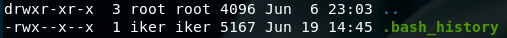
\includegraphics[scale=.75]{ls -la.png} 
\end{center}

\begin{table}[!htb]
\begin{minipage}{.5\linewidth}
      \centering
        \begin{tabular}{|c|c|}
            \hline
            Number & Permissions\\
            \hline
            0 & No permissions\\
            1 & Execute\\
            2 & Write\\
            3 & Write, Execute\\
            4 & Read\\
            5 & Read, Execute\\
            6 & Read, Write\\
            7 & Read, Write, Execute\\
            \hline
        \end{tabular}
    \end{minipage}%
    \begin{minipage}{.5\linewidth}
      \centering
        \begin{tabular}{|c|c|c|}
        	\hline
            User & Group & Others\\
            \hline
            	\begin{tabular}{ccc}-&-&-\end{tabular}&\begin{tabular}{ccc}-&-&-\end{tabular}&\begin{tabular}{ccc}-&-&-\end{tabular}\\
            	\begin{tabular}{ccc}-&-&x\end{tabular}&\begin{tabular}{ccc}-&-&x\end{tabular}&\begin{tabular}{ccc}-&-&x\end{tabular}\\
            	\begin{tabular}{ccc}-&w&-\end{tabular}&\begin{tabular}{ccc}-&w&-\end{tabular}&\begin{tabular}{ccc}-&w&-\end{tabular}\\
            	\begin{tabular}{ccc}-&w&x\end{tabular}&\begin{tabular}{ccc}-&w&x\end{tabular}&\begin{tabular}{ccc}-&w&x\end{tabular}\\
            	\begin{tabular}{ccc}r&-&-\end{tabular}&\begin{tabular}{ccc}r&-&-\end{tabular}&\begin{tabular}{ccc}r&-&-\end{tabular}\\
            	\begin{tabular}{ccc}r&-&x\end{tabular}&\begin{tabular}{ccc}r&-&x\end{tabular}&\begin{tabular}{ccc}r&-&x\end{tabular}\\
            	\begin{tabular}{ccc}r&w&-\end{tabular}&\begin{tabular}{ccc}r&w&-\end{tabular}&\begin{tabular}{ccc}r&w&-\end{tabular}\\
            	\begin{tabular}{ccc}r&w&x\end{tabular}&\begin{tabular}{ccc}r&w&x\end{tabular}&\begin{tabular}{ccc}r&w&x\end{tabular}\\
            	\hline
        \end{tabular}
    \end{minipage} 
\end{table}

\newpage
\section{The System}
\subsection{Color Coded}
\begin{itemize}
\item Blue: Directory.
\item Green: Executable or recognized data file.
\item Sky Blue: Symbolic link file.
\item Yellow with black background: Device
\item Pink: Graphic image file.
\item Red: Archive file.
\item Red with black background: Broken link.
\end{itemize}
\subsection{The Filesystem Hierarchy Standard (FHS)}
\begin{itemize}
\item \textbf{/bin}: Essential user command binaries.
\item \textbf{/etc}: Configuration files for the system.
\item \textbf{/sbin}: Essential system binaries.
\item \textbf{/usr}: Read-only user application support data \& binaries.
\begin{itemize}
\item /usr/bin: Most user commands.
\item /usr/include: Standard include files for C code.
\item /usr/lib: Obj, bin, lib files for coding and packages.
\item /usr/local: Local software (./bin ./lib ./man ./sbin ./share).
\item /usr/share: Static data shareable across all architectures.
\begin{itemize}
\item /usr/share/man: Manual pages.
\end{itemize}
\end{itemize}
\item \textbf{/var}: Variable data files.
\begin{itemize}
\item /var/cache: Application cache data.
\item /var/lib: Data modifies as programmes run.
\item /var/lock: Lock files to track resources in use.
\item /var/log: Log files.
\item /var/opt: Variable data for installed packages.
\item /var/spool: Tasks waiting to be processed:
\begin{itemize}
\item /var/spool/cron
\item /var/spool/cups
\item /var/spool/mail
\end{itemize}
\item /var/tmp: Temporary files saved between reboots.
\end{itemize}
\item \textbf{/dev}: Device files included /dev/null.
\item \textbf{/home}: User home directories.
\item \textbf{/lib}: Libraries \& kernel modules.
\item \textbf{/mnt}: Mount files for temporary filesystems.
\item \textbf{/opt}: Optional software applications.
\item \textbf{/proc}: Process \& kernel information files.
\item \textbf{/root}: Home directory for the root user.
\end{itemize}
\newpage
\end{document}